% results part

\subsection{Image compression}

In \cref{fig:imagecompr} both the original image used as the input data
and the resulting image after the $k$-means clusters had been found
for $k = 24$ and $k = 10$.

\begin{figure}[!ht]
    \centering
    \begin{subfigure}[t]{1\textwidth}
        \centering
        \includegraphics[width=.9\textwidth]{doc/bad-water-good-light-wallpaper.jpg}
        \caption{Before $k$-means compression}
    \end{subfigure}
    \begin{subfigure}[t]{1\textwidth}
        \centering
        \includegraphics[width=.9\textwidth]{doc/out.png}
        \caption{After $k$-means compression with $k = 24$ clusters}
    \end{subfigure}
    \begin{subfigure}[t]{\textwidth}
        \centering
        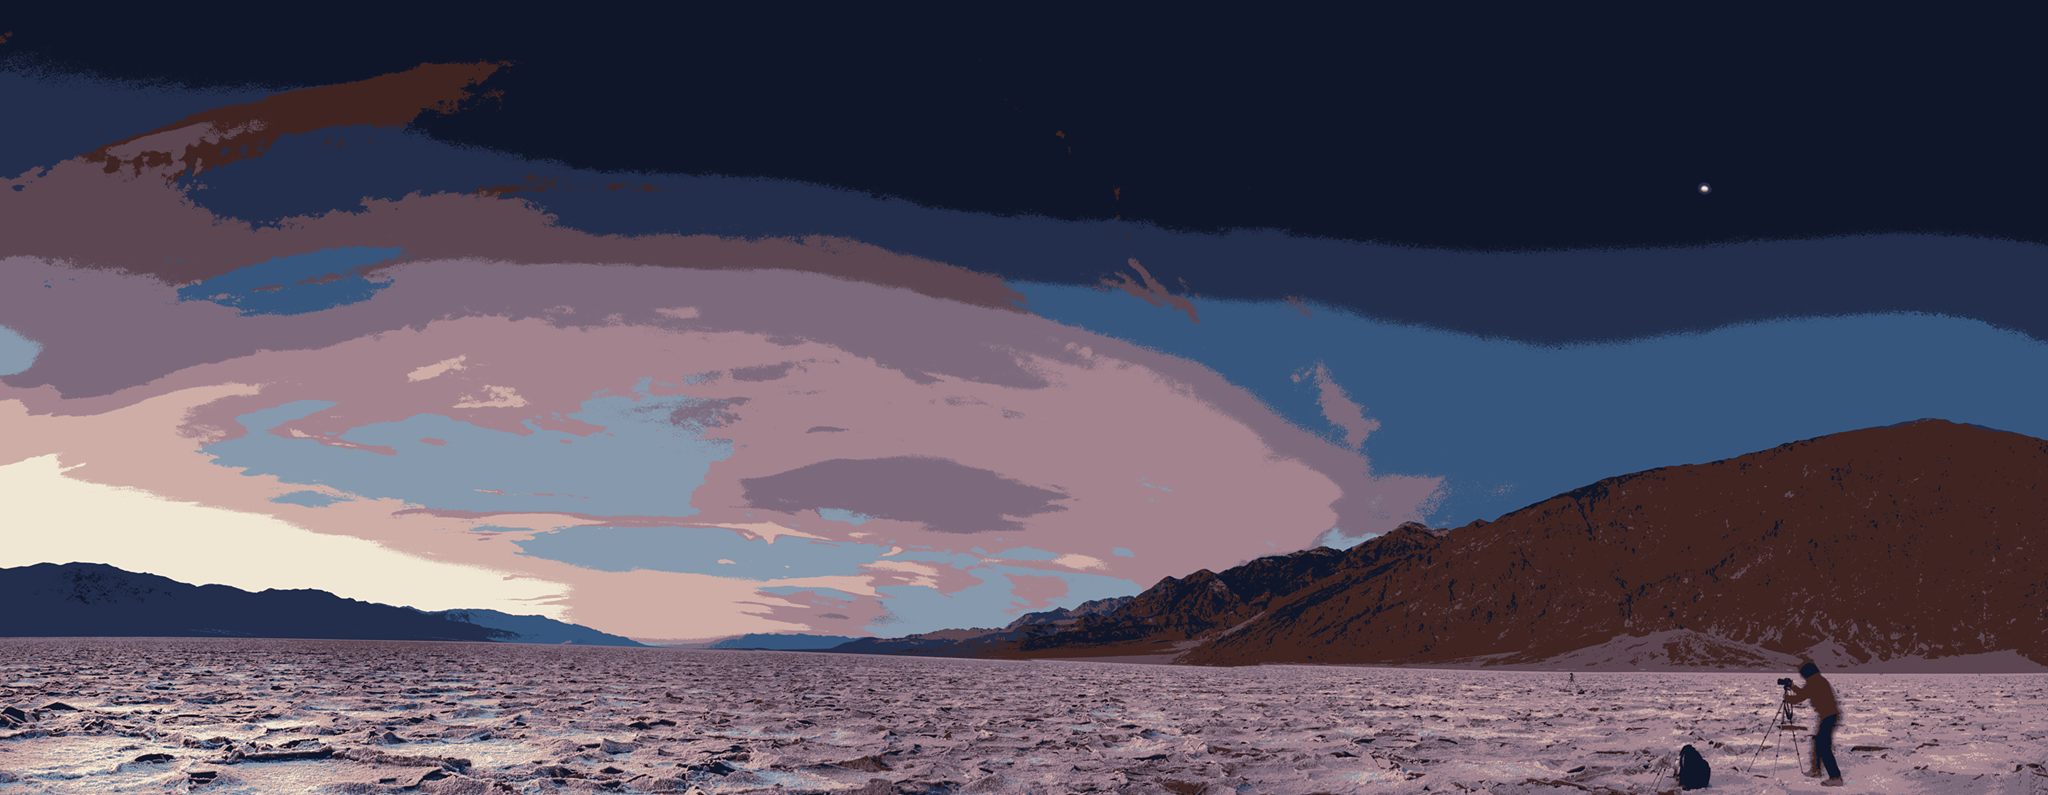
\includegraphics[width=.9\textwidth]{doc/out2.png}
        \caption{After $k$-means clustering with $k = 10$ clusters}
    \end{subfigure}
    \caption{The input image and its outputs after clustering}
    \label{fig:imagecompr}
\end{figure}

\subsection{Computation time}

\Cref{fig:time_read} shows the elapsed time during the computations on the picter done at Tegner
for increasing ammount of processes.
The image seen in \cref{fig:imagecompr} was used as the input for all of the plotted times with $k$ set to 10.
For $p = 1$ the serial version of Lloyd's algorithm, \cref{alg:lloyds}, was used,
while for all $p > 1$ the parallel version, \cref{alg:parlloyds}, were used.
4-5 runs where used for each process setup and used to create a statistical mean and standard deviation,
which are plotted as the area in the figure.
We can see that the computation time decreases in a exponential fashion as expected.

\begin{table}[!ht]
  \centering
  \pgfplotstabletypeset[
    col sep=comma,
    header=true,
    columns={p, tt, tts},
    columns/p/.style={column name=Processes},
    columns/tt/.style={column name=$T_\text{comp}$},
    columns/tts/.style={column name=$\sigma$},
    every head row/.style={before row=\toprule, after row=\midrule},
    every last row/.style={after row=\bottomrule}
  ]{data/results_means_var.csv}
\end{table}

\begin{figure}[!ht]
  \centering
  \begin{subfigure}[t]{0.5\textwidth}
    \centering
    \begin{tikzpicture}
      \begin{axis}[
        xmin=1,
        xmax=22,
        ylabel={t [s]},
        xlabel={p}]
        \addplot+[
          color=blue
        ] table [x=p, y=tt, col sep=comma] {data/results_means.csv};
        \addplot+[
          color=blue,
          name path=hi
        ] table [x index=0, y expr=\thisrowno{3} + \thisrowno{6}, col sep=comma] {data/results_means_var.csv};
        \addplot+[
          color=blue,
          name path=lo
        ] table [x index=0, y expr=\thisrowno{3} - \thisrowno{6}, col sep=comma] {data/results_means_var.csv};
        \addplot+[color=blue, opacity=0.5] fill between [of=hi and lo];
      \end{axis}
    \end{tikzpicture}
    \caption{Total execution time}
    \label{fig:meanvar}
  \end{subfigure}
  ~
  \begin{subfigure}[t]{0.5\textwidth}
    \centering
      \begin{tikzpicture}
        \begin{axis}[
          xmin=1,
          xmax=22,
          ylabel={t [s]},
          xlabel={p}]
          \addplot+[color=blue] table [x=p, y=tc, col sep=comma] {data/results_means.csv};
        \addplot+[
          color=blue,
          name path=hi
        ] table [x index=0, y expr=\thisrowno{2} + \thisrowno{5}, col sep=comma] {data/results_means_var.csv};
        \addplot+[
          color=blue,
          name path=lo
        ] table [x index=0, y expr=\thisrowno{2} - \thisrowno{5}, col sep=comma] {data/results_means_var.csv};
        \addplot+[color=blue, opacity=0.5] fill between [of=hi and lo];
        \end{axis}
      \end{tikzpicture}
    \caption{Execution time for $k$-means parallel}
  \end{subfigure}
  ~
  \begin{subfigure}[t]{0.5\textwidth}
    \centering
      \begin{tikzpicture}
        \begin{axis}[
          xmin=1,
          xmax=22,
          ylabel={t [s]},
          xlabel={p}]
          \addplot+[color=blue] table [x=p, y=tr, col sep=comma] {data/results_means.csv};
        \addplot+[
          color=blue,
          name path=hi
        ] table [x index=0, y expr=\thisrowno{1} + \thisrowno{4}, col sep=comma] {data/results_means_var.csv};
        \addplot+[
          color=blue,
          name path=lo
        ] table [x index=0, y expr=\thisrowno{1} - \thisrowno{4}, col sep=comma] {data/results_means_var.csv};
        \addplot+[color=blue, opacity=0.5] fill between [of=hi and lo];
        \end{axis}
      \end{tikzpicture}
    \caption{Execution time for reading the data in parallel}
  \end{subfigure}
  \label{fig:time_read}
\end{figure}

\begin{figure}[!ht]
  \centering
  \begin{subfigure}[t]{0.5\textwidth}
    \centering
    \begin{tikzpicture}
      \begin{axis}[
        xmin=1,
        xmax=22,
        ylabel={t [s]},
        xlabel={p}]
        \addplot table [x index=0, y index=1, col sep=comma] {data/parallel_speedup.csv};
      \end{axis}
    \end{tikzpicture}
    \caption{Absolute parallel speedup}
  \end{subfigure}
  ~
  \begin{subfigure}[t]{0.5\textwidth}
    \centering
    \begin{tikzpicture}
      \begin{axis}[
        xmin=1,
        xmax=22,
        ylabel={t [s]},
        xlabel={p}]
        \addplot table [x index=0, y index=2, col sep=comma] {data/parallel_speedup.csv};
      \end{axis}
    \end{tikzpicture}
    \caption{Relative parallel speedup}
  \end{subfigure}
  \label{fig:speedup}
\end{figure}
